\documentclass{fhnwreport}
\usepackage[ngerman]{babel}
\usepackage[T1]{fontenc}
\usepackage[utf8]{inputenc}
\usepackage{tikz}
\usetikzlibrary{arrows}
\usepackage{amsmath}
\usepackage{lmodern}
\usepackage[final]{pdfpages}
\usepackage{graphicx}
\usepackage{textcomp}
\usepackage{multirow}
\usepackage{todonotes}
\usepackage{pdfpages}
\bibliographystyle{IEEEtran}
\usepackage{cite}
\usepackage[nottoc,numbib]{tocbibind}

\title{%
  \textsc{Projekt 2}\\[2ex]
  \textsc{Fachbericht}}
\author{%
  \textsc{Team 1}}
\date{%
  \textsc{10.06.2015}}

\begin{document}
\maketitle

\vfill
%\hspace{4em}
\textsc{%
\begin{tabbing}
tab1 \= tab2 \= tab3 \= tab4 \kill
Auftraggeber:  \>\>\>  Peter Niklaus \\[2ex]
Betreuer:  \>\>\>  Pascal Buchschacher, Anita Gertiser \\[2ex]
Experten:  \>\>\>  Peter Niklaus, Richard Gut \\[2ex]
Team:  \>\>\> Alexander Stocker \\ 
\>\>\> Claudius J"org \\
\>\>\> Denis Stampfli \\
\>\>\> Martin Moser \\
\>\>\> Reto Freivogel \\
\>\>\> Yohannes Measho \\ [2ex]
Studiengang: \>\>\> Elektro- und Informationstechnik
\end{tabbing}}

\clearpage
{\Large \textbf{Abstract}}

Regler werden heutzutage oft mit grosszügigen Faustformeln dimensioniert. Für stabilere Regelungen kann die aufwändige Phasengangmethode angewendet werden. Das Ziel dieser Arbeit ist es mit einem Programm die Phasengangmethode stark zu vereinfachen. Die Vereinfachung besteht aus der Eingabe von Werten der identifizierten Strecke und gibt dimensionierte Werte aus. Zusätzlich kann das Programm die Resultate mit verschiedenen Faustformeln vergleichen. Der Fachbericht setzt sich zusammen aus einem mathematischen und einem programmtechnischen Teil. Der mathematische Abschnitt behandelt die Streckenanalyse, die Phasengangmethode und ihr Ablauf, die Übertragungsfunktion der Regler, die Schrittantwort der Regelung und die Optimierungsmöglichkeiten. Er geht auch auf die Dimensionierung mit Faustformeln ein. Der programmtechnische Bericht erläutert die Software, die Benutzerschnittstelle und die Anwendung von Model-View-Controller.


\newpage
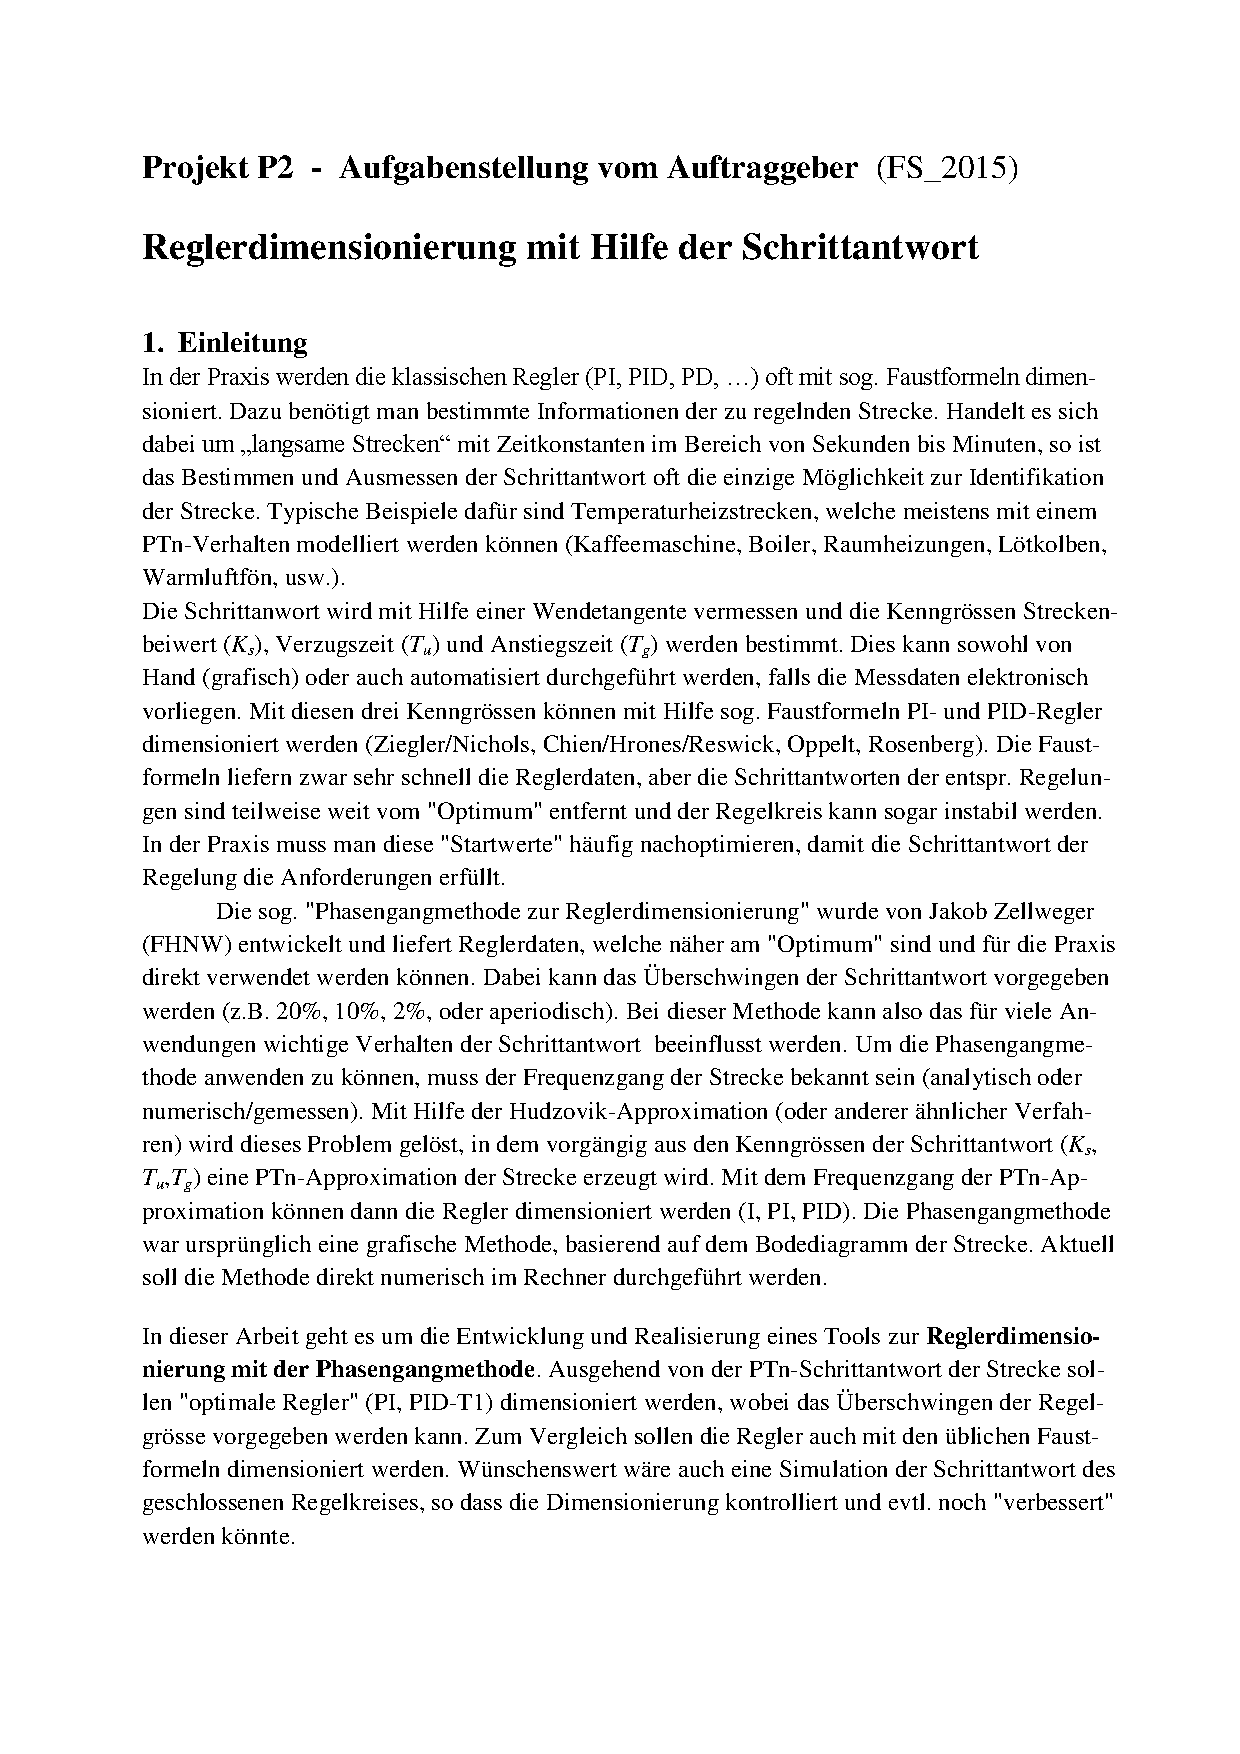
\includepdf[pages=1-2]{aufgabenstellung.pdf}

\newpage
\tableofcontents
\newpage

\section{Einleitung}

\section{Theoretische Grundlagen}
Eine Regelung besteht, wie in Abbildung \ref{regelstrecke} zu sehen ist, aus einem Regler und einer Regelstrecke. Beispiele einer Regelung sind Raumheizungen, Lötkolben oder Geschwindigkeitsregelungen.\newline 

\begin{figure}[h]
\centering
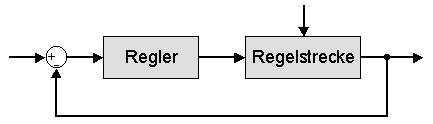
\includegraphics[width=0.8\textwidth]{Regelstrecke.png}
\caption{Regelung bestehend aus Regler und Regelstrecke}
\label{regelstrecke}
\end{figure}
%Quelle: http://rn-wissen.de/wiki/index.php/Datei:Regelkreis4.png [Abrufdatum 6.5.15]


Ist eine Regelstrecke gegeben, im Falle eines Lötkolbens wäre dies die Distanz vom Heizelement bis zur Lötspitze, so muss ein dazu passender Regler dimensioniert werden. Reglerdimensionierungen können über das Auswerten der Schrittantwort der Regelstrecke durchgeführt werden. Um die Schrittantwort zu erhalten wird das Verhalten der Strecke aufgrund eines Schrittes der Eingangsgrösse gemessen. Für die Berechnungen werden die aus der Schrittantwort der Strecke ausgelesenen Kenngrössen Verzugszeit ($T_u$), Anstiegszeit ($T_g$) und Streckenbeiwert ($K_s$) verwendet. Zur Dimensionierung eines passenden Reglers existieren verschiedenste Methoden. Im Folgenden werden nun zwei Möglichkeiten genauer erläutert, wobei das Hauptaugenmerk auf der ersten Methode, der Phasengangmethode, liegt und die zweite, die Dimensionierung mittels gängigen Faustformeln, lediglich zum Vergleich durchgeführt wird.\newline

\newpage
Die Kurve in Abbildung \ref{schrittantwort} stellt die Schrittantwort einer Regelstrecke dar. Daran angelegt ist die Wendetangente, die benötigt wird, um die Verzugs- und die Anstiegszeit messen zu können.\newline

\begin{figure}[h]
\centering
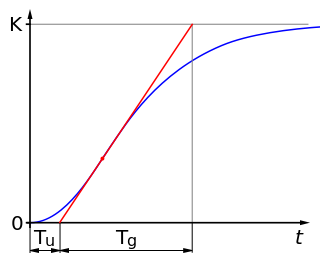
\includegraphics[width=0.6\textwidth]{Schrittantwort.png}
\caption{Schrittantwort einer Regelstrecke}
\label{schrittantwort}
\end{figure}
%Quelle: http://de.wikipedia.org/wiki/Faustformelverfahren_%28Automatisierungstechnik%29#/media/File:Tutg.svg [Abrufdatum 6.5.15]

Ziel ist es, PI- sowie PID-Regler zu dimensionieren, das heisst deren Kennwerte zu berechnen. Der PI-Regler hat die Kennwerte Nachstellzeit ($T_n$) und Reglerverstärkung ($K_R$), beim PID-Regler kommt noch die Vorhaltezeit ($T_v$) hinzu.



\subsection{Streckenanalyse}
Die Streckenidentifikation wird mittels der Sani-Methode durchgeführt. Aus dem Verhältnis von $T_u$ und $T_g$ werden die Ordnung der Strecke und die dazugehörigen Zeitkonstanten berechnet, die benötigt werden, um die Übertragungsfunktion der Regelstrecke darzustellen. \newline 


% Quelle Skript "Mathematisches Labor mlab", Soenicki/Bürgi
Die Übertragungsfunktion der Strecke ist gemäss Formel \ref{ufunkstr} definiert:

\begin{align}
G_S(s)=\frac{K_S}{(1+sT_1)(1+sT_2)...(1+sT_n)}
\label{ufunkstr}
\end{align}

\newpage
\subsection{Phasengangmethode}
Bei der Phasengangmethode handelt es sich eigentlich um eine grafische Dimensionierungsmethode, welche früher noch von Hand mit logarithmischem Papier durchgeführt wurde. Anstelle der grafischen Dimensionierung wird die Methode in diesem Fall komplett rechnerisch gelöst. Um die Methode zu verstehen wird ein theoretisches Grundwissen benötigt, welches in folgenden Unterkapiteln erklärt wird.


\subsubsection{Grundlagen}
Durch Ersetzen von $s$ durch $j\omega$ in der Übertragungsfunktion der Strecke erhält man den Frequenzgang. Um die Phasengangmethode anwenden zu können, wird der Amplituden- und Phasengang der Regelstrecke benötigt.
% Vielleicht noch ein Satz zur Definition a-gang ph-gang, wie man auf die Formeln kommt


\begin{align}
A_S(\omega)=abs(G_S(j\omega))
\end{align}
\begin{align}
\varphi_S(\omega)=arg(G_S(j\omega))
\end{align}
\begin{align}
\varphi_S(\omega)=-arctan(\omega T_1)-arctan(\omega T_2)...-arctan(\omega T_n)
\end{align}\newline

Die Zeitkonstanten des zu dimensionierenden Reglers stehen in direktem Zusammenhang mit dessen Amplitudengang. In den Abbildungen \ref{agangpi} und \ref{agangpid} sind die Amplitudengänge eines PI- und eines PID-Reglers dargestellt, wobei die x-Achsen logarithmisch skaliert sind. Wie die Kreisfrequenzen an den Knickstellen mit den Reglerparametern zusammenhängen sollen, ist in Tabelle \ref{amplitudengaenge} ersichtlich.\newline

\begin{figure}[h]
\centering
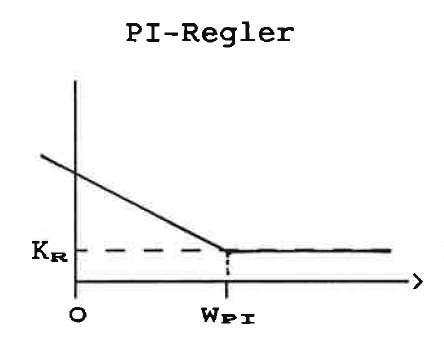
\includegraphics[width=0.5\textwidth]{agangpi.png}
\caption{Amplitudengang PI-Regler Amp($\omega$) (log. Darstellung)}
\label{agangpi}
\end{figure}
%Quelle: Zellwegerskript

\begin{figure}[h]
\centering
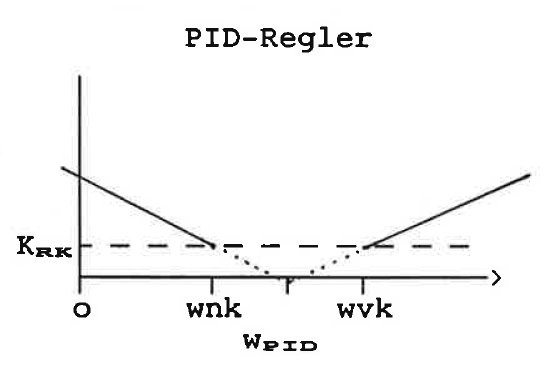
\includegraphics[width=0.6\textwidth]{agangpid.png}
\caption{Amplitudengang PID-Regler Amp($\omega$) (log. Darstellung)}
\label{agangpid}
\end{figure}
%Quelle: Zellwegerskript

\begin{table}[h]
\centering
\renewcommand*{\arraystretch}{1.7}
\begin{tabular}{|l|l|c|}
\hline 
\textbf{PI-Regler} & \multicolumn{2}{c|}{\textbf{PID-Regler}} \\ 
\hline 
$\omega_{PI}=\frac{1}{T_n}$ & $\omega_{nk}=\frac{1}{T_{nk}}=\beta*\omega_{PID}$ & $\omega_{vk}=\frac{1}{T_{vk}}=\frac{\omega_{PID}}{\beta}$ \\ 
\hline 
\end{tabular}
\caption[Amplitudengänge / Knickkreisfrequenzen]{Amplitudengänge Regler und Zusammenhänge mit Knickkreisfrequenzen}
\label{amplitudengaenge}
\renewcommand*{\arraystretch}{1} 
\end{table}

\newpage
Diese Knickkreisfrequenzen werden mithilfe des Phasengangs der Strecke berechnet. Je nach dem welcher Reglertyp dimensioniert werden soll, müssen andere Punkte im Phasengang gesucht werden (Tabelle \ref{phgangpunkte}).\newline

\begin{table}[h]
\centering
\renewcommand*{\arraystretch}{1.7}
\begin{tabular}{|l|c|c|}
\hline 
\textbf{Regler} & \textbf{Phasengang der Strecke $\varphi_s$} & \textbf{Knickkreisfrequenz}  \\ 
\hline 
\textbf{PI} & $-\frac{\pi}{2}=-90^\circ$ & $\omega_{PI}=\frac{1}{T_n}$ \\ 
\hline 
\textbf{PID} & $-\frac{3\pi}{4}=-135^\circ$ & $\omega_{PID}=\frac{1}{\sqrt{T_{nk}T_{vk}}}$ \\ 
\hline 
\end{tabular}
\caption[Wichtige Phasengangpunkte]{Gesuchte Punkte im Phasengang je nach Regler}
\label{phgangpunkte}
\renewcommand*{\arraystretch}{1} 
\end{table}

\newpage
Der PI-Regler kann anhand dieser Dimensionierungskriterien bereits dimensioniert werden. Beim PID-Regler muss allerdings noch ein Parameter mehr bestimmt werden. Es handelt sich um den Faktor $\beta$ welcher benötigt wird um die Knickkreisfrequenzen des PID-Reglers berechnen zu können. Dieser Faktor $\beta$ hängt mit der Tangentensteigung des Phasengangs der offenen Regelung im Punkt $-135^\circ$ zusammen.\newline
Ein Dimensionierungskriterium der Phasengangmethode lautet, dass die Steigung des Phasengangs der gesamten, offenen Regelung bei der Knickkreisfrequenz $\frac{-0.5}{\omega_{PID}}$ betragen soll. Dies hat damit zu tun, dass eine Steigung von -20dB/Dekade angestrebt wird. Die genaue Herleitung von $\beta$ befindet sich im Anhang. \newline

Es gilt also die folgende Beziehung:\newline

\begin{align}
\frac{2\beta}{1+\beta^2} + \omega_{PID}\frac{d\varphi_{Strecke(\omega_{PID})}}{d\omega} = -0.5
\end{align}\newline

Da der Phasengang der Strecke und somit dessen Ableitung gegeben ist, kann durch Auflösen nach $\beta$ nun auch dieser Parameter ermittelt werden. Ergibt sich ein Wert grösser als eins oder imaginär, so wird $\beta$ als eins angenommen.

Die Verstärkung des Reglers wird mit Hilfe des Phasenrands bestimmt. Der Phasenrand ist die Differenz der Streckenphase zu $-180^\circ$. Bei unterschiedlichem Phasenrand ergeben sich unterschiedliche Verstärkungsfaktoren, was auch auf das Überschwingen des Reglers Einfluss hat. Tabelle \ref{phasenrand} zeigt den Zusammenhang zwischen dem gewählten Phasenrand und dem daraus resultierenden Überschwingen der Regelung.\newline


\begin{table}[h]
\centering
\renewcommand*{\arraystretch}{1.2}
\begin{tabular}{|c|c|c|}
\hline 
\textbf{Phasenrand $\varphi_R$} & \textbf{Streckenphase $\varphi_S$} & \textbf{Überschwingen} \\ 
\hline 
$45^\circ$ & $-135^\circ$ & $23\%$ \\ 
\hline 
$51.8^\circ$ & $-128.5^\circ$ & $16.3\%$ \\ 
\hline 
 $65.5^\circ$& $-114.6^\circ$ & $4.6\%$ \\ 
\hline 
$76.3^\circ$ & $-103.7^\circ$ & $0\%$ \\ 
\hline
\end{tabular} 
\caption{Zusammenhang Phasenrand und Überschwingen}
\label{phasenrand}
\renewcommand*{\arraystretch}{1}
\end{table}

\newpage
Zur Berechnung der Verstärkung werden nun die Amplitudengänge der Strecke, sowie des Reglers benötigt. Die Werte dieser beiden Amplitudengänge an der Stelle wo der Phasenrand abgetragen wurde, werden miteinander multipliziert. Gemäss Phasengangmethode soll die Verstärkung an dieser Stelle eins sein. Dies führt zur Formel \ref{formelkr}:\newline
\begin{align}
K_R=\frac{1}{\vert{Go(\omega_D)}\vert{}}
\label{formelkr}
\end{align}


\subsubsection{Ablauf der Phasengangmethode}
Die Phasengangmethode der Strecke $\varphi_S$ wird nach dem folgenden Ablauf durchgeführt. Die Punkte 2. und 3. werden nur für PID-Regler benötigt. Eine numerische Beispielrechnung für einen PI-Regler ist im Anhang angefügt.
\begin{enumerate}
\item Im Phasengang der Strecke $\varphi_S$ werden die Kreisfrequenzen in bestimmten Punkten gesucht.
\item Der Faktor $\beta$ wird bestimmt.
\item Mithilfe von $\beta$ werden die Zeiten $T_{nk}$ und $T_{vk}$ ermittelt.
\item Der Phasengang der offenen Regelung $\varphi_{go}$ wird berechnet (Phasengang Strecke + Phasengang Regler)
\item Die Kreisfrequenz $\omega_D$ beim gewählten Phasenrand wird berechnet.
\item Die Amplitudengänge der Strecke sowie des Reglers bei $\omega_D$ werden miteinander multipliziert. Damit wird die Reglerverstärkung $K_R$ festgelegt. 
\end{enumerate}

Besondere Vorsicht ist bei den erhaltenen Kenngrössen des dimensionierten Reglers geboten. Es wird zwischen Regler- und Bodekonform unterschieden. Bodekonform bedeutet, dass die Parameter kaskadiert sind und die logarithmische Rechnung somit vereinfacht wird. Standardmässig wird in der Fachliteratur meist reglerkonform gerechnet. Die Parameter des PI-Reglers sind reglerkonform und können somit direkt weiterverwendet werden. Die Parameter des PID-Reglers, welche wir bei der Dimensionierung mittels Phasengangmethode erhalten, sind bodekonform. Sie können jedoch in die reglerkonforme Darstellung umgerechnet werden. Für die Umrechnung wurden die Formeln \ref{krherl}, \ref{tnherl} und \ref{tvherl} für PID-Regler hergeleitet (siehe Anhang): \newline


\begin{align}
K_R=K_{rk}\left(1+\frac{T_{vk}}{T_{nk}}-\frac{T_p}{T_{nk}}\right)
\label{krherl}
\end{align}
\begin{align}
T_n=T_{nk}+T_{vk}-T_p
\label{tnherl}
\end{align}
\begin{align}
T_v=\frac{T_{nk}T_{vk}}{T_{nk}+T_{vk}-T_p}-T_p
\label{tvherl}
\end{align}\newline

Tp steht für die parasitäre Zeitkonstante. Diese wird benötigt, da ein idealer PID-Regler in der Praxis nicht umsetzbar ist. Der Index k in der bodekonformen Darstellung steht für Kaskadierung.

\subsection{Übertragungsfunktion der Regler}
Um schlussendlich die Schrittantwort der geschlossenen Regelung berechnen zu können, wird die Übertragungsfunktion des dimensionierten Reglers benötigt. Diese lässt sich mit den aus der Phasengangmethode erhaltenen Parametern aufstellen (Tabelle \ref{ufunkregler}).\newline
\begin{table}
\centering
\renewcommand*{\arraystretch}{1.7}
\begin{tabular}{|l|l|}
\hline 
\textbf{Beschreibung} & \textbf{Darstellung} \\ 
\hline
PI-Regler bodekonform & $G_R(s)=K_R\frac{(1+sT_n)}{sT_n}$ \\ 
\hline 
PI-Regler reglerkonform & $G_R(s)=K_R\left(1+\frac{1}{sT_n}\right)$ \\ 
\hline 
PID-Regler bodekonform & $G_R(s)=K_{rk}\frac{(1+sT_{nk})(1+sT_{vk})}{sT_{nk}(1+sT_p)}$ \\ 
\hline 
PID-Regler reglerkonform & $G_R(s)=K_R\left(1+\frac{1}{sT_n}+\frac{sT_v}{1+sT_p}\right)$ \\ 
\hline 
\end{tabular} 
\renewcommand*{\arraystretch}{1}
\caption{Übertragungsfunktionen Regler}
\label{ufunkregler}
\end{table}

\newpage
\subsection{Dimensionierung mit Faustformeln}
Die Dimensionierung mittels Faustformeln wird durchgeführt, um die Dimensionierungsresultate der Phasengangmethode am Schluss zu vergleichen und auszuwerten. Es gibt etliche verschiedene Faustformeln von unterschiedlichen Personen. Die bekanntesten und gängigsten Dimensionierungsformeln sind in den folgenden Tabellen aufgelistet und werden im Programm implementiert.\\

\begin{table}[h]
\centering
\renewcommand*{\arraystretch}{1.7}
\begin{tabular}{|l|l|c|c|c|}
\hline 
\textbf{Formeltyp} & \textbf{Regler} & \textbf{$K_R$} & \textbf{$T_n$} & \textbf{$T_v$} \\ 
\hline 
 & \textbf{P} & $\frac{T_g}{K_sT_u}$ &  &  \\ 
\cline{2-5} 
\textbf{Ziegler/Nichols}&\textbf{PI} & $\frac{0.9*T_g}{K_sT_u}$ & $3.3*T_u$ &  \\ 
\cline{2-5} 
&\textbf{PID} & $\frac{0.9*T_g}{K_sT_u}$ & $2*T_u$ & $0.42*T_t$ \\ 
\hline 

&\textbf{P} & $\frac{T_g}{K_sT_u}$ &  &  \\ 
\cline{2-5} 
\textbf{Oppelt} &\textbf{PI} & $\frac{0.8*T_g}{K_sT_u}$ & $3*T_u$ &  \\ 
\cline{2-5} 
&\textbf{PID} & $\frac{1.2*T_g}{K_sT_u}$ & $2*T_u$ & $0.42*T_t$ \\ 
\hline 

&\textbf{P} & $\frac{T_g}{K_sT_u}$ &  &  \\ 
\cline{2-5} 
\textbf{Rosenberg} &\textbf{PI} & $\frac{0.91*T_g}{K_sT_u}$ & $3.3*T_u$ &  \\ 
\cline{2-5}  
&\textbf{PID} & $\frac{1.2*T_g}{K_sT_u}$ & $2*T_u$ & $0.44*T_t$ \\ 
\hline 

\end{tabular} 
\renewcommand*{\arraystretch}{1}
\caption{Fausformeln Ziegler/Nichols, Oppelt und Rosenberg}
\end{table}

\begin{table}
\centering
\renewcommand*{\arraystretch}{1.5}
\begin{tabular}{|l|c|c|c|c|}
\hline 
& \multicolumn{2}{c|}{\textbf{aperiodischer}} & \multicolumn{2}{c|}{\textbf{Einschwingvorgang mit}} \\
\textbf{Reglertyp} & \multicolumn{2}{c|}{\textbf{Einschwingvorgang}} & \multicolumn{2}{c|}{\textbf{20\% Überschwingen}}\\
\cline{2-5} 
 & Führung & Störung & Führung & Störung \\ 
\hline 
\textbf{P} & $K_R=\frac{0.3*T_g}{K_sT_u}$ & $K_R=\frac{0.3*T_g}{K_sT_u}$ & $K_R=\frac{0.7*T_g}{K_sT_u}$ & $K_R=\frac{0.7*T_g}{K_sT_u}$ \\ 
\hline 
\multirow{2}{*}{\textbf{PI}} & $K_R=\frac{0.35*T_g}{K_sT_u}$ & $K_R=\frac{0.6*T_g}{K_sT_u}$ & $K_R=\frac{0.6*T_g}{K_sT_u}$ & $K_R=\frac{0.7*T_g}{K_sT_u}$ \\ 
& $T_n=1.2*T_g$ & $T_n=4*T_u$ & $T_n=T_g$ & $T_n=2.3*T_u$ \\ 
\hline 
 & $K_R=\frac{0.6*T_g}{K_sT_u}$ & $K_R=\frac{0.95*T_g}{K_sT_u}$ & $K_R=\frac{0.95*T_g}{K_sT_u}$ & $K_R=\frac{1.2*T_g}{K_sT_u}$\\ 
\textbf{PID} & $T_n=T_g$ & $T_n=2.4*T_u$ &  $T_n=1.35*T_g$ & $T_n=2.3*T_u$ \\ 
 & $T_v=0.5*T_u$ & $T_v=0.42*T_u$ & $T_v=0.47*T_u$ & $T_v=0.42*T_u$ \\ 
\hline 
\end{tabular}
\renewcommand*{\arraystretch}{1}
\caption{Chien/Hrones und Reswick} 
\end{table}


\newpage
\subsection{Schrittantwort der Regelung}
- Übertragungsfunktion Regelung (Berechnung aus üfunk regler und üfunk regelung)\newline
- Berechnung durch Residuen\newline

Um die Schrittantwort der geschlossenen Regelung berechnen zu können, wird die Übertragungsfunktion der Regelung benötigt. Diese wird aus den Übertragungsfunktionen des Reglers und der Strecke gemässe Formel \ref{ufunkregelung} berechnet.

\begin{align}
G(s)=\frac{G_R(s)G_S(s)}{1+G_R(s)G_S(s)}
\label{ufunkregelung}
\end{align}


\section{Software}
\textbf{Hinweise zur Benutzung}\\
Der Fachbericht dient zur Erklärung des Aufbaus des Java Source Codes. Für eine Einführung in das Programm beachte man die Bedienungsanleitung im Anhang.\\
\textit{JavaKlassenNamen} sind im Folgenden kursiv mit Grossbuchstaben geschrieben. Dagegen sind \textit{packages} kursiv und klein geschrieben. Das gesamte Klassendiagramm befindet sich im Anhang.\\
Fett gedruckte Nummern (\textbf{1}) beziehen sich auf Elemente des GUIs. Eine Abbildung des GUIs mit Nummerierung findet sich am Ende der Bedienungsanleitung im Anhang.\\

\textbf{Ziele}\\
Ziel der Applikation ist die automatische Dimensionierung eines Reglers mit der Phasengangmethode von Prof. J. Zellweger. Weiter soll die Schrittantwort des gesamten Regelkreises ermittelt und visualisiert werden. Die Regelstrecke ist durch die Parameter $K_s$, $T_u$ und $T_g$ gegeben. Neben der Phasengangmethode sind auch Faustregeln zur Reglerdimensionierung anwendbar. Die berechneten Werte sowie die markanten Werte der Schrittantwort sollen als Text ausgegeben werden. Die Software verfügt weiter über die nützlichen Befehle Rückgängig und Wiederholen. Die eingegebenen Werte können zudem gespeichert und geladen werden.\\

\textbf{Aufbau und Packages}\\
Die Applikation ist nach dem Model-View-Controller Architekturmuster aufgebaut. Wiedergespiegelt ist das in den drei Packages \textit{model}, \textit{view} und \textit{controller}.\\
Das \textit{model} soll eine Abstraktion der mathematischen Objekte bieten. Die meisten enthaltenen Klassen sind für die Vermeidung von Aliasing-Problemen (Zugriff zweier Klassen auf die gleiche Instanz) als unveränderlich gehalten.\\
Die Klassen zur Reglerdimensionierung sind für die bessere Kapselung im separaten Package \textit{model.dimensionierung} enthalten. Alle Klassen dieses Packages sind als unveränderlich gehalten.\\
Das \textit{view} erzeugt die graphische Benutzeroberfläche mit den Daten des \textit{models}. Die Kommunikation zwischen \textit{view} und \textit{model} erfolgt mittels dem Observer Entwurfsmuster.\\
Der \textit{controller} übernimmt die Steuerung der Applikation und die Ausführung der Befehle des Benutzers. 


\newpage
\subsection{Packages und seine Klassen}

\subsubsection{Klassen des Packages \textit{controller}}
Der Aufbau des Packages \textit{controller} ist in Abbildung \ref{packcontrl} ersichtlich.\\

\textit{\textbf{Controller}}\\
Der \textit{Controller} ist verantwortlich für die Steuerung der Applikation. Er besitzt für alle Befehle die der Benutzer im GUI tätigen kann eine Methode zur Modifizierung des \textit{Models}. Meldet das \textit{Model} beim Modifizieren einen Fehler informiert er den Benutzer mit der Methode displayError des \textit{Views}. Vor jeder Änderung des \textit{Models} speichert sich der \textit{Controller} eine Kopie davon. Dadurch ist es möglich alte Zustände wiederherzustellen und die Befehle Rückgängig und Wiederholen zu unterstützen. Weiter ist der \textit{Controller} für das Speichern und Laden zuständig. Dies funktioniert da das \textit{Model} das \textit{Serializable} Interface implementiert und der \textit{Controller} so die Daten mit einem \textit{ObjectOutputStream} in eine Datei schreiben bzw. mit einem \textit{ObjectInputStream} aus einer Datei laden kann.\\

\textit{\textbf{PIDRechner}}\\
Diese Klasse ist der Startpunkt (main) der Applikation. Sie initialisiert \textit{Controller}, \textit{View} und \textit{Model}.

\begin{figure}[p]
\centering
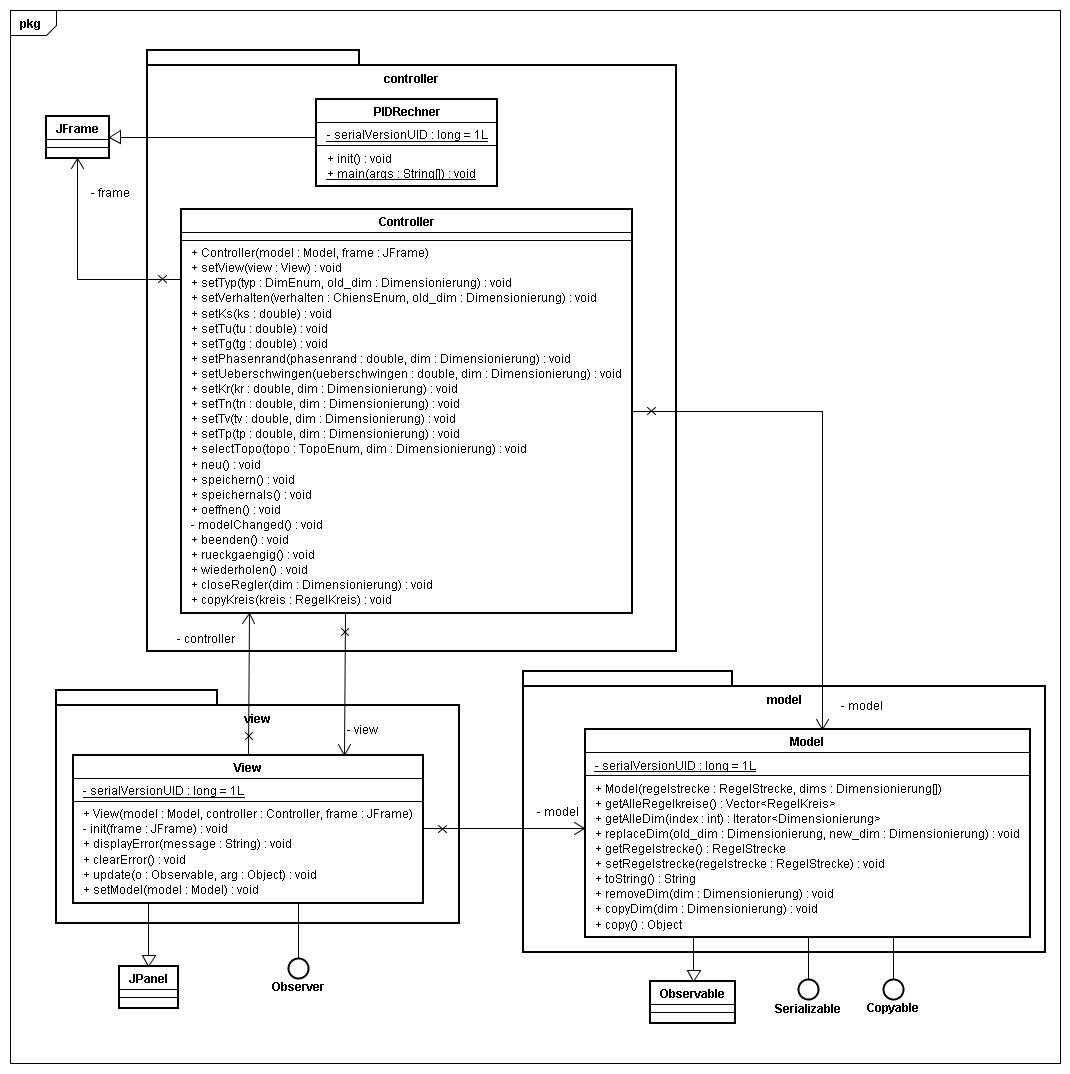
\includegraphics[width=1\textwidth]{packcontrl.png}
\caption{Package \textit{controller}}
\label{packcontrl}
\end{figure}

\newpage
\subsubsection{Ausgewählte Klassen des Packages \textit{model}}
Der Aufbau des Packages \textit{model} ist in Abbildung \ref{packmodel} ersichtlich.\\

\textit{\textbf{Model}}\\
Das \textit{Model} verwaltet die \textit{Regelstecke} und die verschiedenen \textit{Dimensionierungen}. Es bietet Zugriffsmethoden um die \textit{Regelstrecke} und \textit{Dimensionierungen} zu modifizieren. Auch kann es Dimensionierungsmethoden kopieren oder löschen.\\

\textit{\textbf{Regelkreis}}\\
Die Klasse \textit{Regelkreis} dient zur Umwandlung der Übertragungsfunktionen (\textit{TransferFunction}) von Regelstrecke und Regler in die Übertragungsfunktion des ganzen Kreises.\\

\textit{\textbf{Regelstrecke}}\\
Die Klasse \textit{Regelstrecke} bietet eine Abstraktion einer PTn-Strecke mit den Attributen $K_s$, $T_u$ und $T_g$. Eine \textit{Regelstrecke} ist ein \textit{Regelglied}, das heisst sie kann als eine Übertragungsfunktion angesehen werden. Die Übertragungsfunktion wird durch die Sani-Approximation (\textit{SaniApprox}) gebildet.\\

\textit{\textbf{Regler}}\\
Diese Klasse dient zur Abstraktion eines PID-T Reglers mit den Parametern $K_R$, $T_n$, $T_v$ und $T_p$. Ein \textit{Regler} wird normalerweise durch eine Dimensionierungsmethode (\textit{Dimensionierung}) gebildet.\\

\textit{\textbf{TransferFunction}}\\
Eine Übertragungsfunktion besteht aus Zähler- und Nenner-\textit{Polynom}. Sie bietet Methoden zur Faltung und Berechnung der Residuen. Weiter kann aus jeder Übertragungsfunktion eine \textit{Schrittantwort} gebildet werden.\\

\textit{\textbf{Polynom}}\\
\textit{Polynom} abstrahiert reelle Polynome beliebigen Grades. Es bietet Methoden zur Addition und Multiplikation mit anderen \textit{Polynomen}. Weiter können die Wurzeln und die Residuen (mit einem angenommenen Zähler von 1) ausgelesen werden. \\
 
\textit{\textbf{Schrittantwort}}\\
Die Klasse \textit{Schrittantwort} stellt die Schrittantwort für ein lineares \textit{Regelglied} ohne Durchgriff dar. Sie bietet zudem Methoden zur Analyse. So kann sie feststellen ob eine Schrittantwort ausschwingt und wie gross An- und Ausschwingzeit sind. Weiter sucht sie nach dem Maximalwert der Kurve und bietet die Möglichkeit dessen Zeitpunkt und Grösse auszulesen.

\begin{figure}[p]
\centering
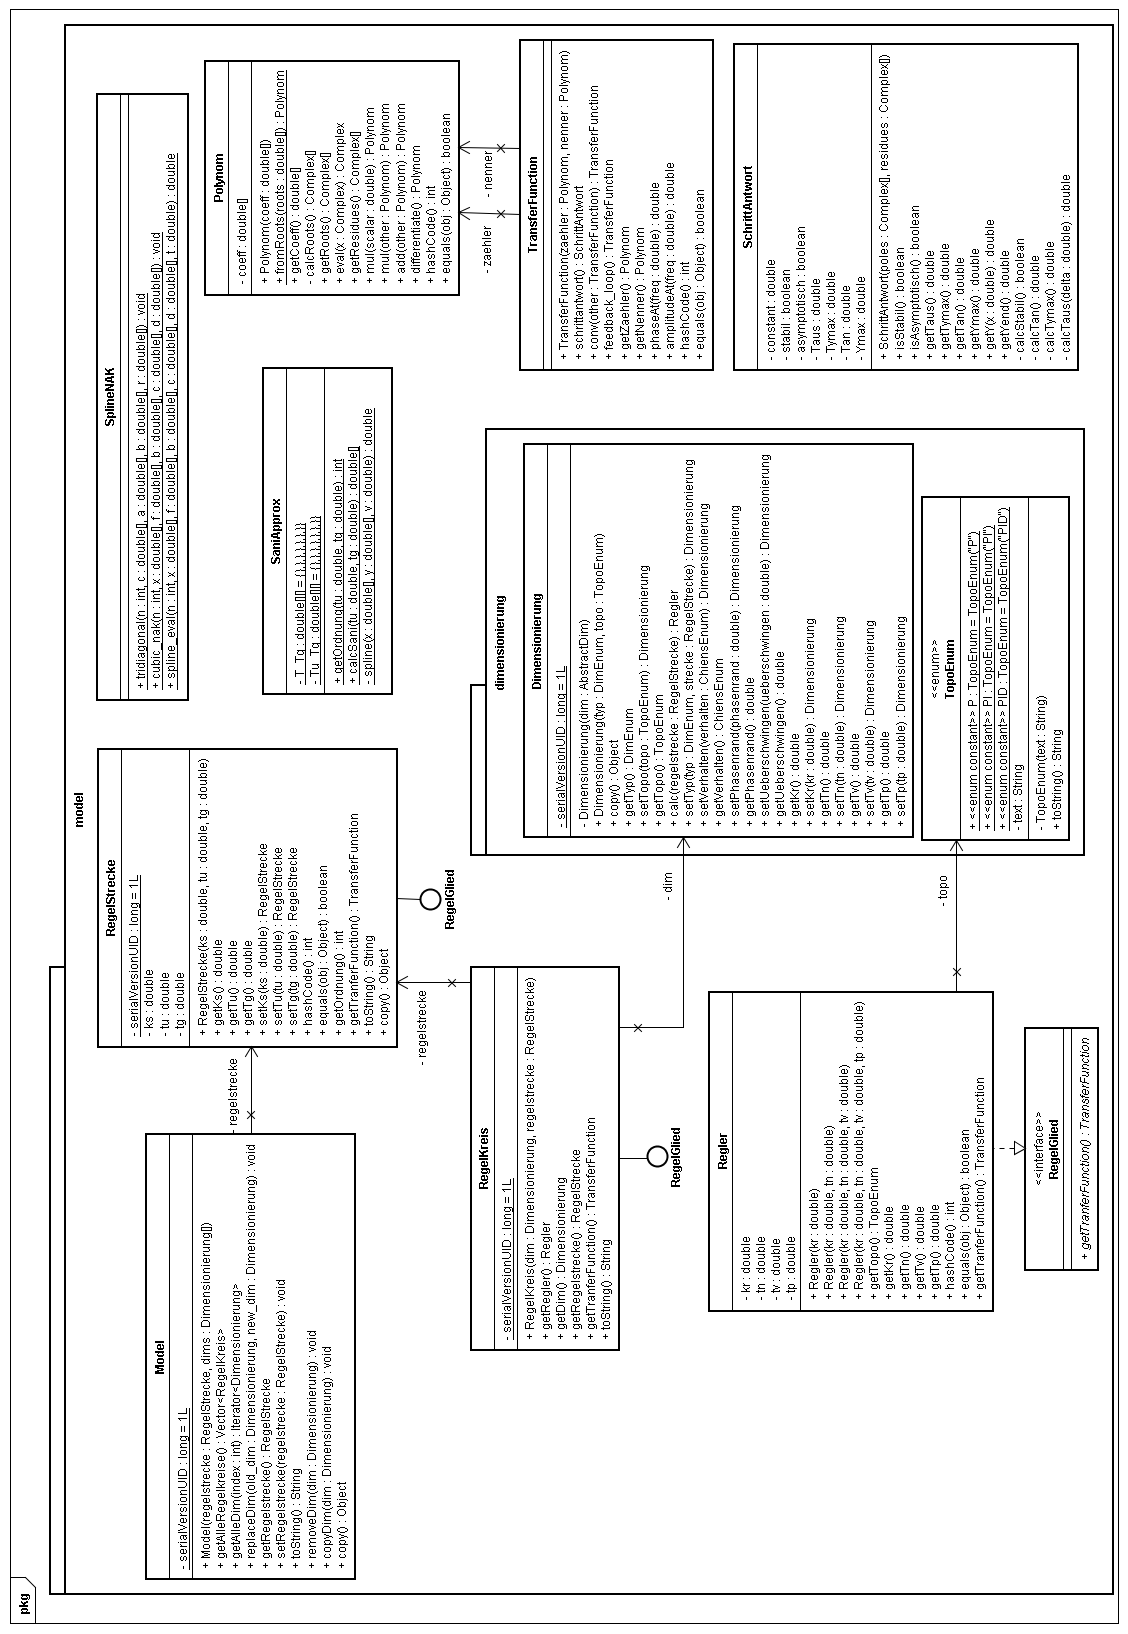
\includegraphics[width=1\textwidth]{packmodel.png}
\caption{Package \textit{model}}
\label{packmodel}
\end{figure}

\newpage
\subsubsection{Ausgewählte Klassen des Packages \textit{dimensionierung}}
Der Aufbau des Packages \textit{dimensionierung} ist in Abbildung \ref{packdim} ersichtlich.\\

\textit{\textbf{Dimensionierung}}\\
Diese Klasse ist eine Auswahl der anderen Dimensionierungsarten, wobei immer nur eine Dimensionierungsart aktiv ist. So bietet diese Klasse auch alle Methoden der anderen Dimensionierungsmethoden. Wird eine Methode bei einer falschen Variante verwendet, wirft die Klasse eine \textit{ClassCastException}. Der Typ (\textit{DimEnum}) kann mit der Methode setTyp gewechselt werden. Beim Wechseln zu der Manuellen Dimensionierungsmethode, werden die Werte des dimensionierten Reglers übernommen.\\

\textit{\textbf{DimEnum}}\\
Dieser Enum dient zur Aufzählung aller Dimensionierungstypen. Er ordnet jedem Typ auch einen Text zu.\\

\textit{\textbf{TopoEnum}}\\
Zur Unterscheidung von PI- und PID-Reglern wird dieser Enum verwendet.\\

\textit{\textbf{AbstractDim}}\\
\textit{AbstractDim} ist die abstrakte Grundklasse aller Dimensionierungsmethoden. Die Methode calc berechnet für eine gegebene Regelstrecke einen Regler. Durch get- und setTopo lässt sich die Reglertopologie (\textit{TopoEnum}) modifizieren. Die Methode getTyp() gibt den Typ des konkreten \textit{Reglers} zurück.\\

\textit{\textbf{ZellwegerDim}}\\
Hier steckt die Phasengangmethode zur Reglerdimensionierung. Die Beschreibung der Methode findet sich im theoretischen Teil.\\

\textit{\textbf{IterativDim}}\\
Diese Methode führt die Phasengangmethode (\textit{ZellwegerDim}) mehrmals nacheinander aus und sucht mit einer binären Suchmethode nach dem gewünschten Überschwingen der Schrittantwort.\\

Die restlichen Klassen entsprechen den verschiedenen Faustregeln.

\begin{figure}[p]
\centering
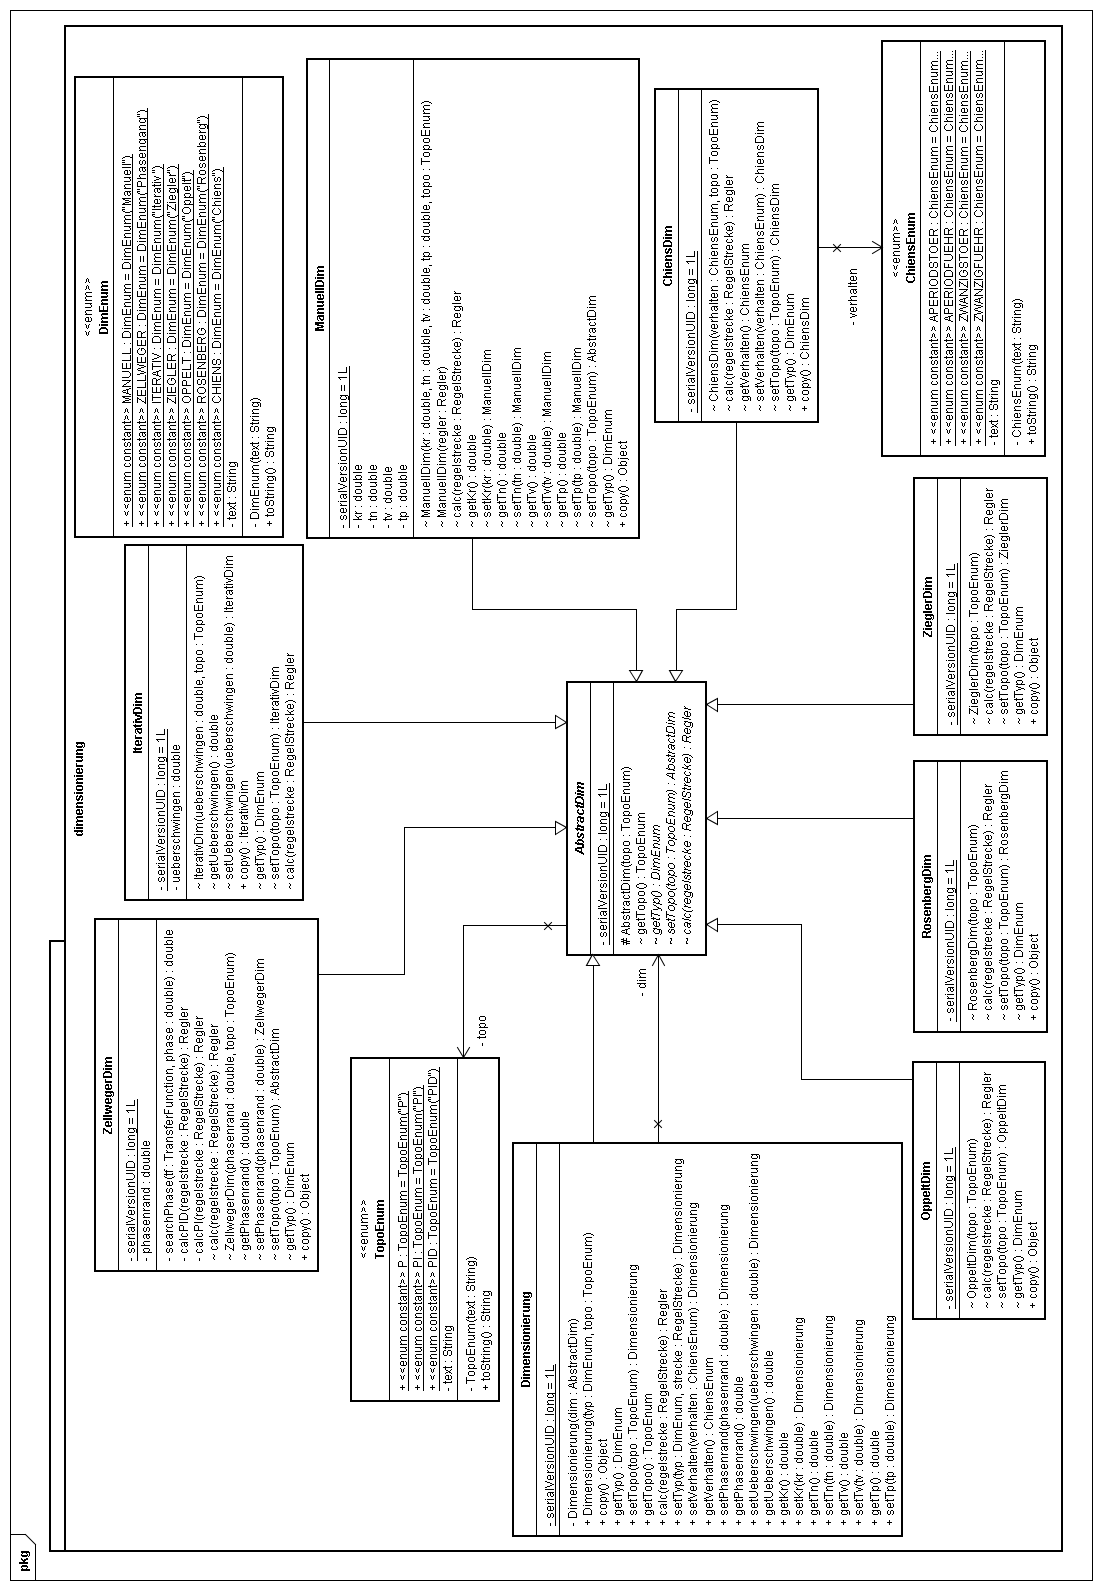
\includegraphics[width=1\textwidth]{packdim.png}
\caption{Package \textit{dimensionierung}}
\label{packdim}
\end{figure}

\newpage
\subsubsection{Klassen des Packages \textit{view}}
Der Aufbau des Packages \textit{view} ist in Abbildung \ref{packview} ersichtlich.\\

\textit{\textbf{View}}\\
\textit{View} ist die oberste Ebene im GUI (abgesehen vom \textit{JFrame}). Es beheimatet die \textit{Sidebar}, den \textit{Graph} und die Statuszeile. Auch initialisiert es die Menübar vom \textit{JFrame}.\\

\textit{\textbf{SidebarPanel}}\\
\textit{SidebarPanel} ordnet die einzelnen Panels von \textit{RegelstreckeView}, \textit{ReglerView} und \textit{AnalyseView} vertikal untereinander an. Es können mehrere Instanzen von \textit{ReglerView} angezeigt werden.\\

\textit{\textbf{RegelstreckeView}}\\
\textit{RegelstreckeView} zeigt die Parameter der \textit{Regelstrecke} sowie die berechnete Ordnung und die Zeitkonstanten an.\\

\textit{\textbf{ReglerView}}\\
Dieses \textit{JPanel} visualisiert den Typ der Dimensionierungsmethode, deren Parameter und die Werte des daraus resultierenden \textit{Reglers}.\\

\textit{\textbf{AnalyseView}}\\
Listet die Eigenschaften Anstiegszeit ($T_{an}$), Ausschwingzeit ($T_{aus}$), Maximalwert ($Y_{max}$) und Zeitpunkt des Maximalwertes ($T_{Ymax}$) der \textit{Schrittantwort} auf.\\

\textit{\textbf{Graph}}\\
Zeichnet alle \textit{Schrittantworten} mit der Klasse \textit{ChartPanel} von JFreeChart. Unter dem Graphen zeigt es weiter eine Legende. Die Zustände der \textit{Checkboxen} werden nur vom Graph selbst verwendet und nicht dem \textit{Controller} mitgeteilt.

\begin{figure}[p]
\centering
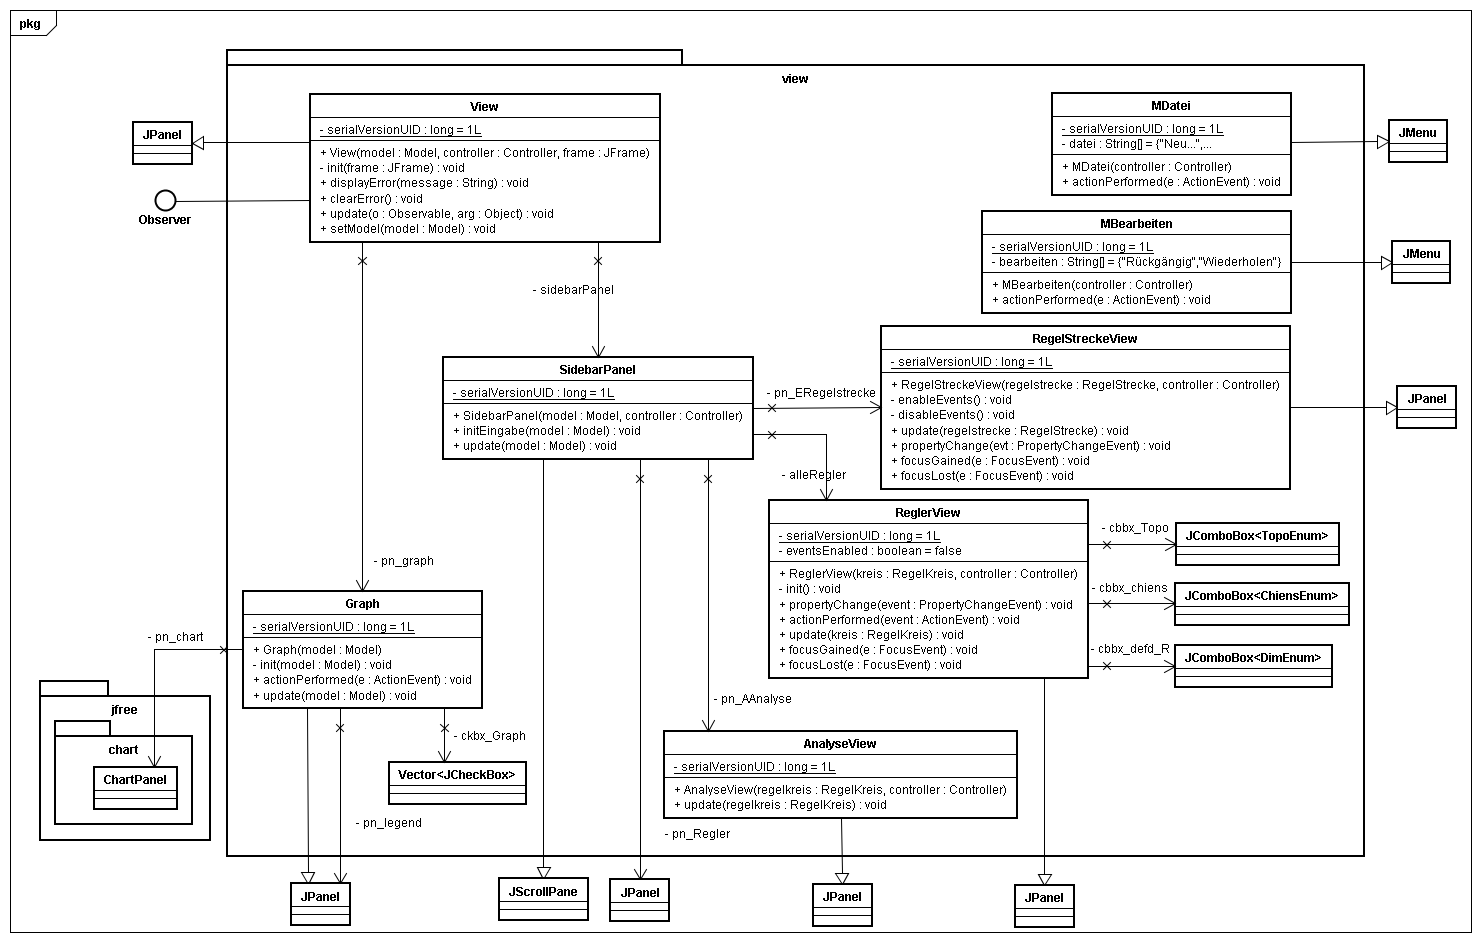
\includegraphics[width=0.9\textwidth]{packview.png}
\caption{Package \textit{view}}
\label{packview}
\end{figure}


\section{Schlusswort}
Ein Software welche auf dem MVC-Pattern aufgebaut ist das Ergebnis am Ende des Projektes. Die Streckenparameter können in der Software eingegeben werden und es resultieren die Parameter des Reglers mit der Schrittantwort der Regelungsstrecke. Die Schrittantwort der Regelung wird unmittelbar vermasst und die Vermassungswerte werden im Analyse Panel dargestellt. Da die Reglerparamter über die Sanimethode berechnet werden, können die Zeiten der Sanimethode ausgewählt werden. Damit verschiedene Regler verglichen werden können, besteht die Möglichkeit, mehrere Plots zu generieren. Das Ziel einfache Bedienung haben wir mit einer übersichtlichen Darstellung und geeigneten Tastenkombinationen realisiert.
Im Grossen und Ganzen haben wir die gesetzten Ziele erreicht. Die Idee hinter der Monte-Carlo Analyse war es, eine Regelung zu berechnen, welche die prozentuale Abweichung graphisch darstellte. Die Eingabewerte der Strecke sollten dabei in einem Range von fünf Prozent tausendmal berechnet werden. Doch aus zeitlichen Gründen konnte dieses Ziel nicht realisiert werden.

\bibliography{literaturverzeichnis}


\newpage
\section{Anhang}
\begin{itemize}
\item Herleitungen Formeln
\item Beispielberechnung Phasengangmethode mithilfe von Matlab
\item Bedienungsanleitung des Programmes
\todo{Alle Anhänge aufführen!!!}
\end{itemize}
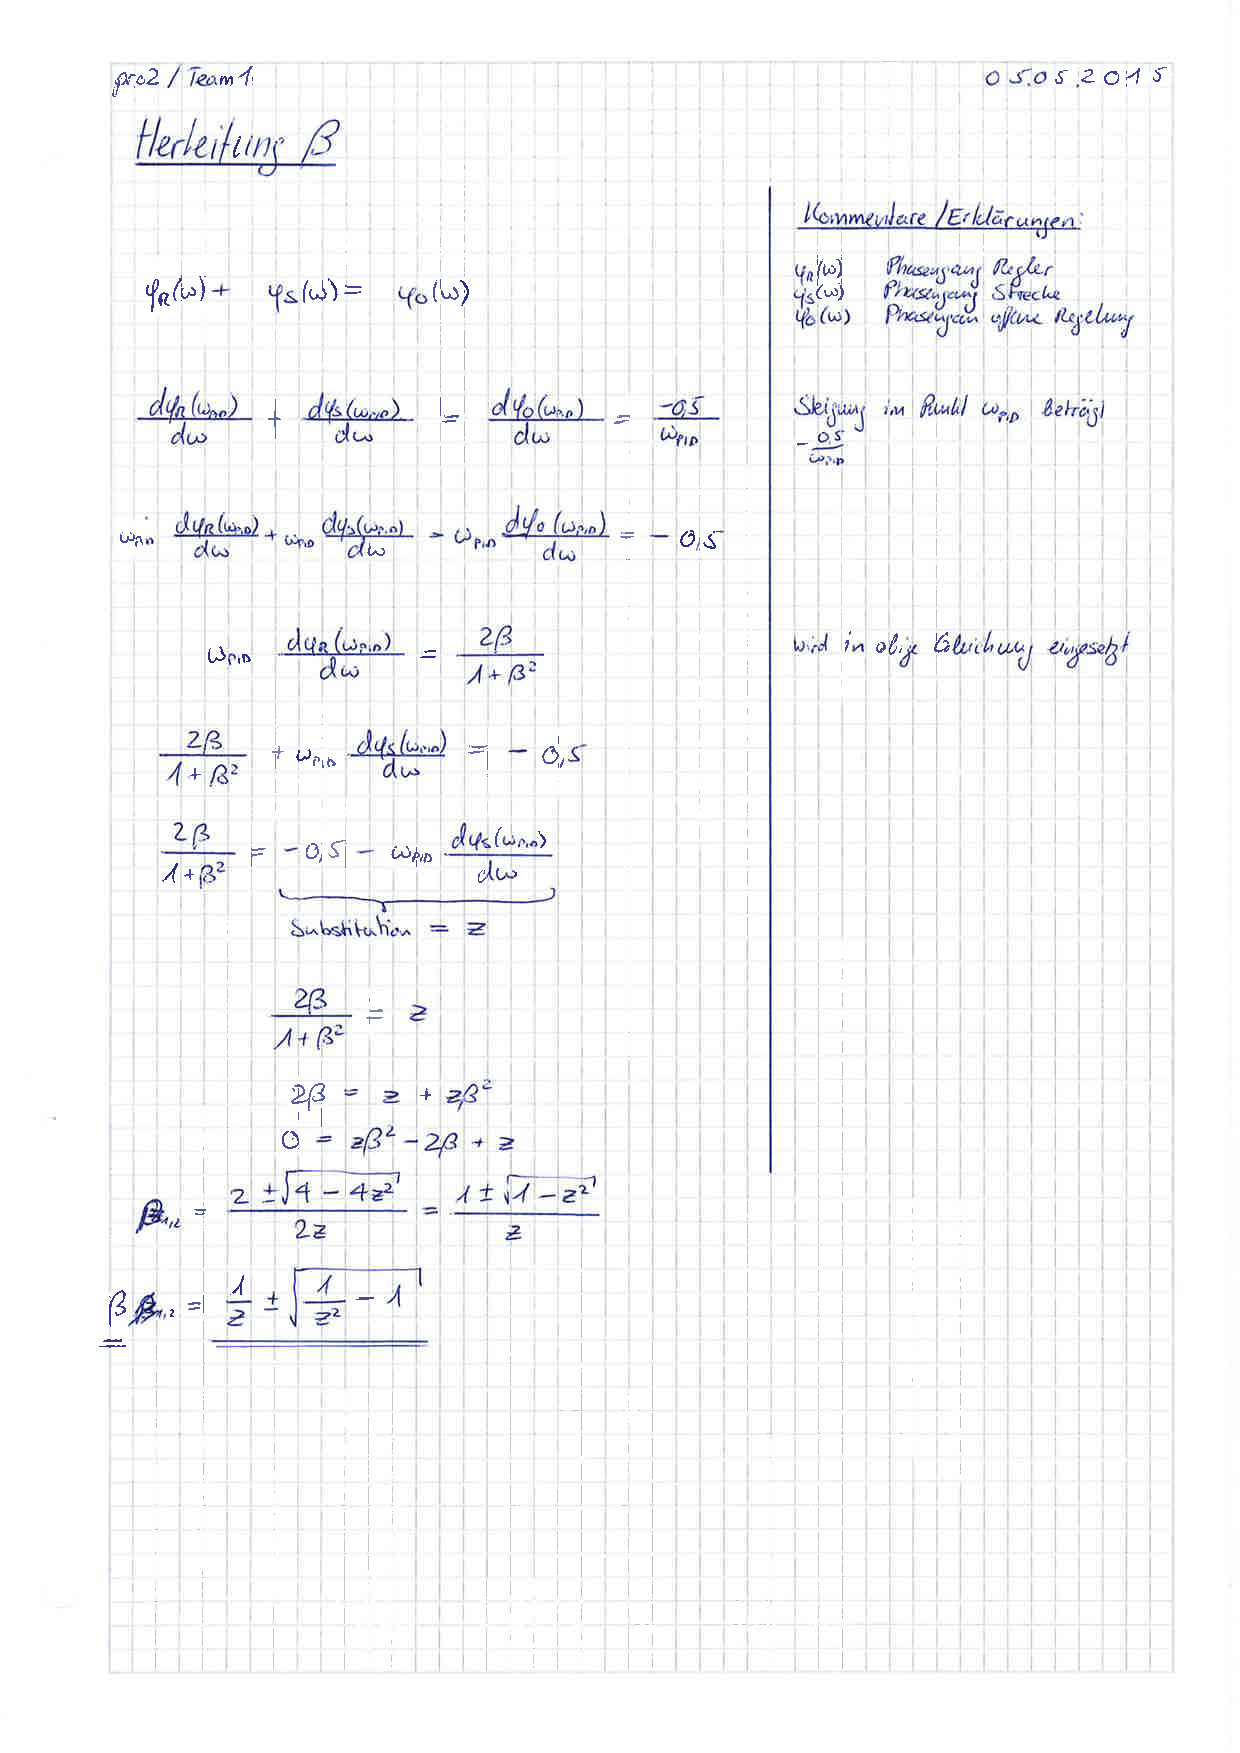
\includepdf[pages=1-2]{Herleitungen_Anhang.pdf}
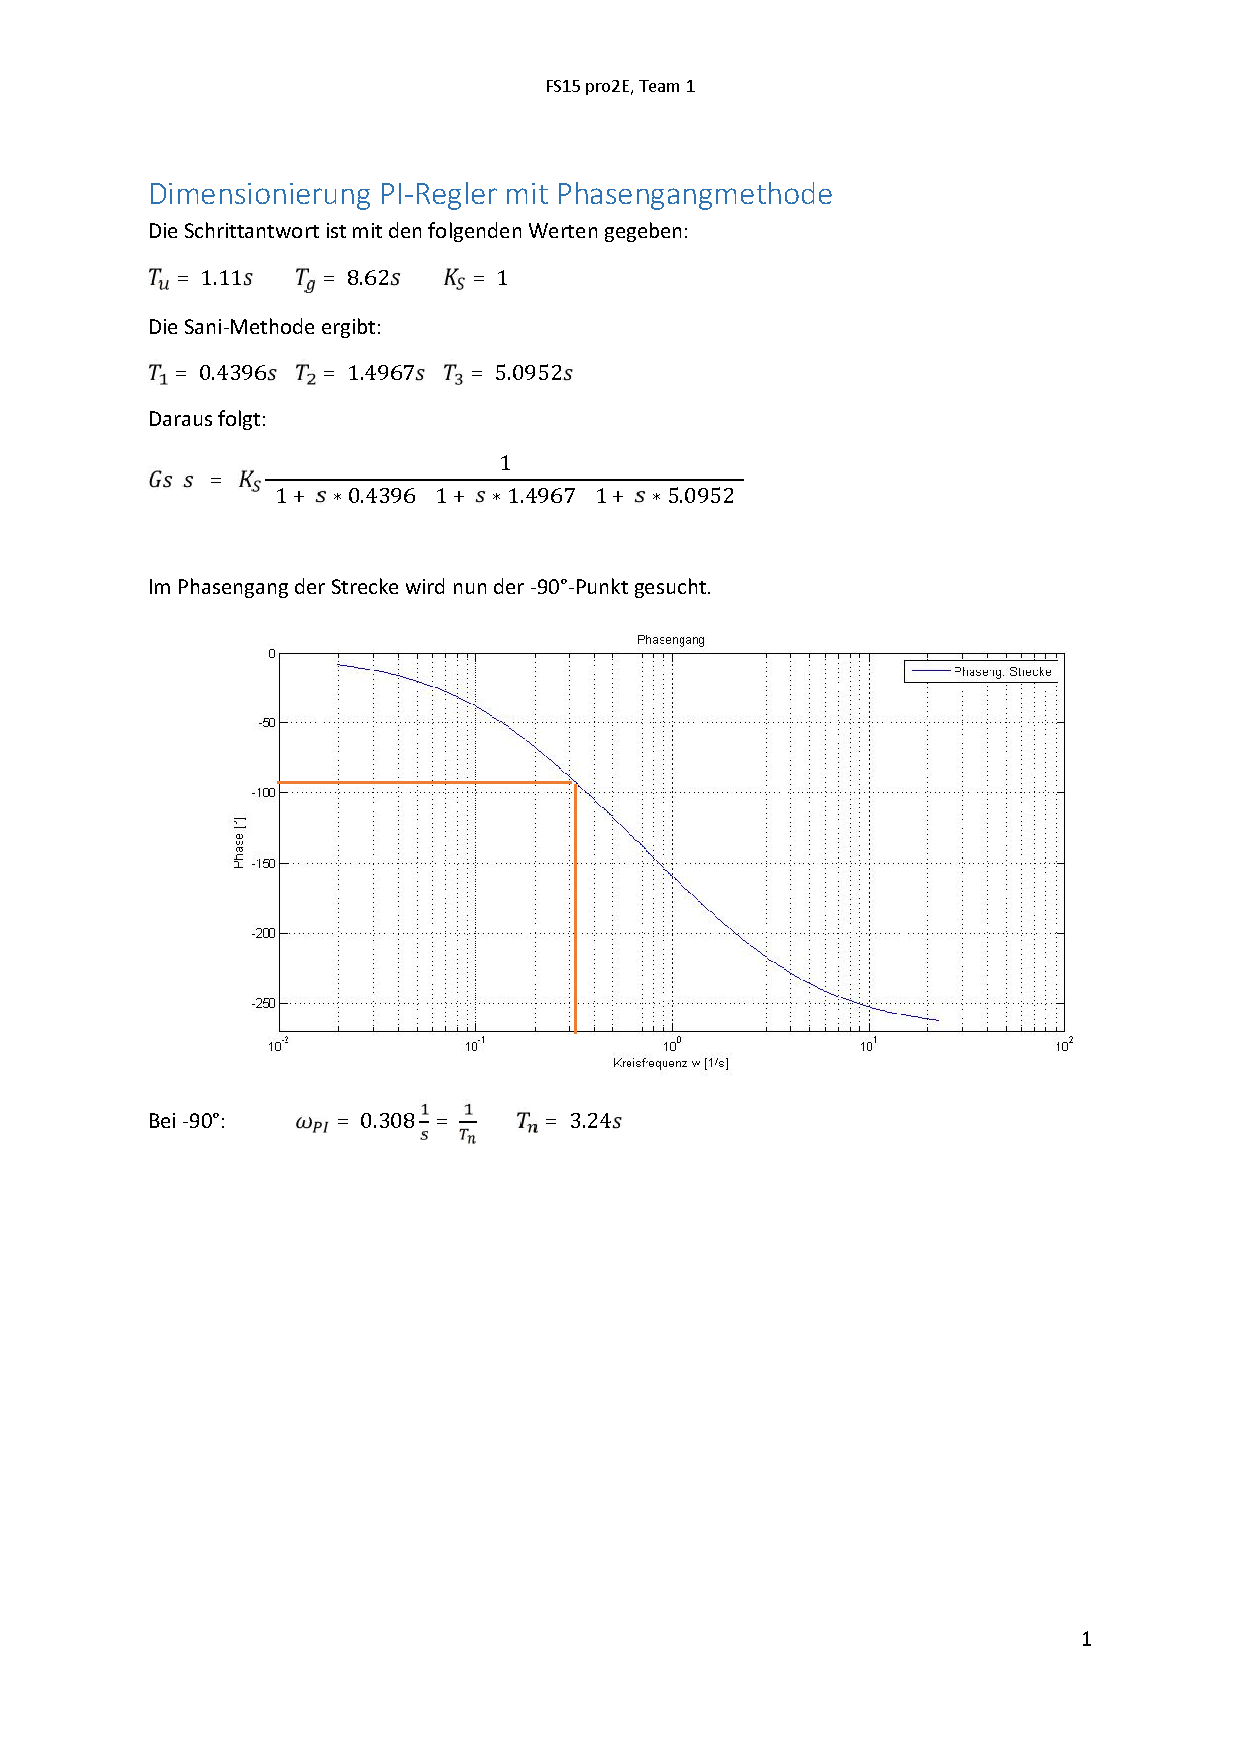
\includepdf[pages=1-3]{Matlab_bsp_berechnung_Anhang.pdf}
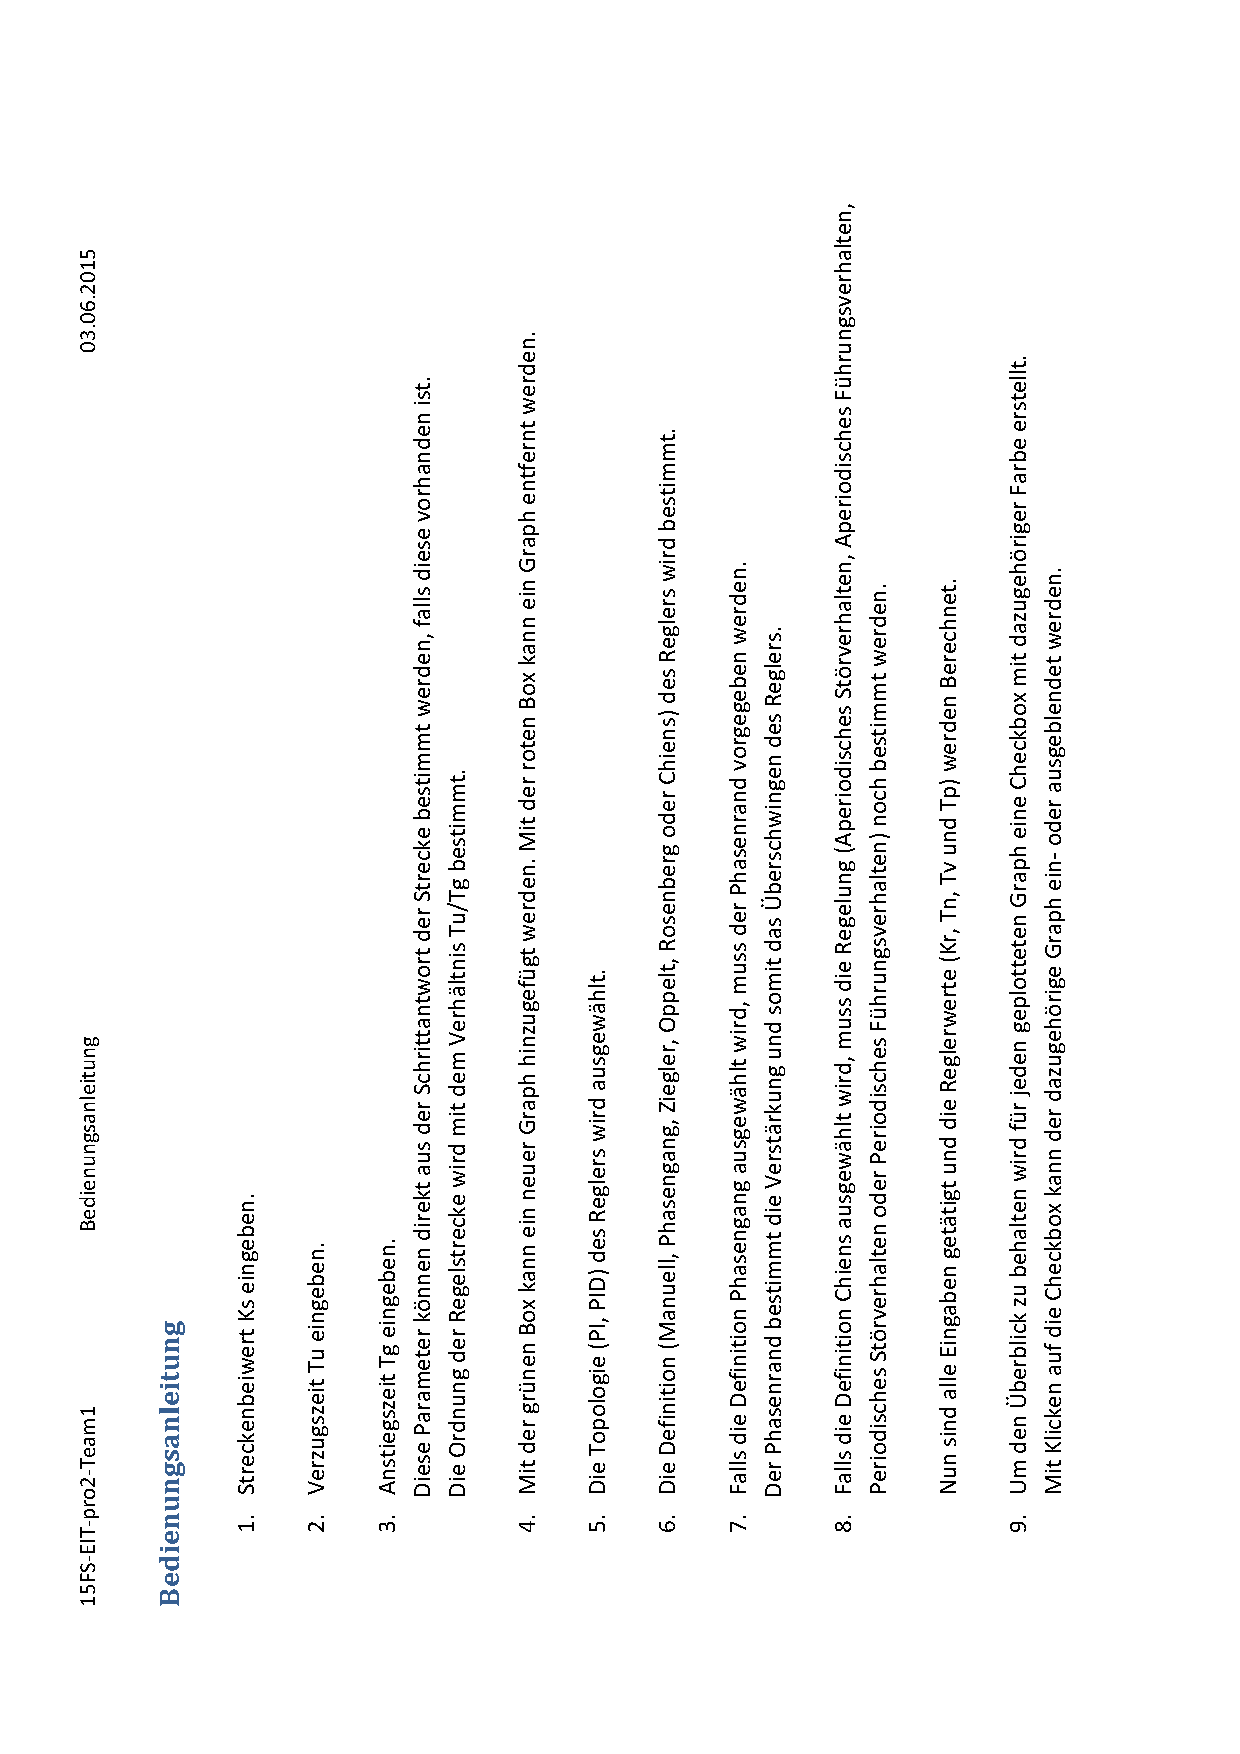
\includepdf[pages=1-2]{Bedienungsanleitung.pdf}

\end{document}

